%%%%%%%%%%%%%%%%%%%%%%%%%%%%%%%%%%%%%%%%%
% Simple Sectioned Essay Template
% LaTeX Template
%
% This template has been downloaded from:
% http://www.latextemplates.com
%
% Note:
% The \lipsum[#] commands throughout this template generate dummy text
% to fill the template out. These commands should all be removed when 
% writing essay content.
%
%%%%%%%%%%%%%%%%%%%%%%%%%%%%%%%%%%%%%%%%%

%----------------------------------------------------------------------------------------
%	PACKAGES AND OTHER DOCUMENT CONFIGURATIONS
%----------------------------------------------------------------------------------------

\documentclass[12pt]{article} % Default font size is 12pt, it can be changed here

\usepackage{geometry} % Required to change the page size to A4
\geometry{a4paper} % Set the page size to be A4 as opposed to the default US Letter

\usepackage{graphicx} % Required for including pictures
\usepackage{pdfpages}
\usepackage{float} % Allows putting an [H] in \begin{figure} to specify the exact location of the figure
\usepackage{wrapfig} % Allows in-line images such as the example fish picture
\usepackage{float}
\usepackage{lipsum} % Used for inserting dummy 'Lorem ipsum' text into the template

\linespread{1.2} % Line spacing

%\setlength\parindent{0pt} % Uncomment to remove all indentation from paragraphs

\graphicspath{{Pictures/}} % Specifies the directory where pictures are stored

\begin{document}


%----------------------------------------------------------------------------------------
%	TITLE PAGE
%----------------------------------------------------------------------------------------


\includepdf[page={1}]{title}
%----------------------------------------------------------------------------------------
%	TABLE OF CONTENTS
%----------------------------------------------------------------------------------------

\tableofcontents % Include a table of contents

\newpage % Begins the essay on a new page instead of on the same page as the table of contents 

%----------------------------------------------------------------------------------------
%	INTRODUCTION
%----------------------------------------------------------------------------------------

\section{Introduction} % Major section
The main topic of this project is to provide a set of visualization tools regarding environmental data collected by a station located in the territory.\\
The requirement is to design three different information visualization tools, which are the following:
\begin{itemize}
\item Individual: app for smartphone/smartwatch
\item Public: ambient display
\item Technical: application for large tablets or desktop
\end{itemize}
Each of the representation is linked by a different type of user, for example the desktop application is made for  letting back end technical personnel  staff to access data at different levels of granularity, instead of the public representation that will provide an approximation of the data collection for letting not technical people understand what they're seeing.\\
\section{Data}
The station will collect the following environmental data:
\begin{itemize}
\item CO2
\item Air Humidity
\item Luminosity
\item Wind speed and direction 
\item Location (also height, type of soil, type of surrounding environment)
\item Time (hour/season)
\item Pressure
\item Rain
\item Temperature
\section{Competitive analisys}
\subsection{Personal interface}
Before we could actualy start the design, a little research on the argument had to be done, about the data representation techniques which could be used with the data we have to visualize and some examples of application which dealed with something similar.

We found some good examples and took some hints.
\subsubsection{Air visual}
This was a good app to start the competitive analysis, because it was the most complete and the prettiest.
We deduced from this app we can organize the general look of the application as a n card view, and there was some historic data management we found vey interesting.
\begin{figure}[H]
  \centering
  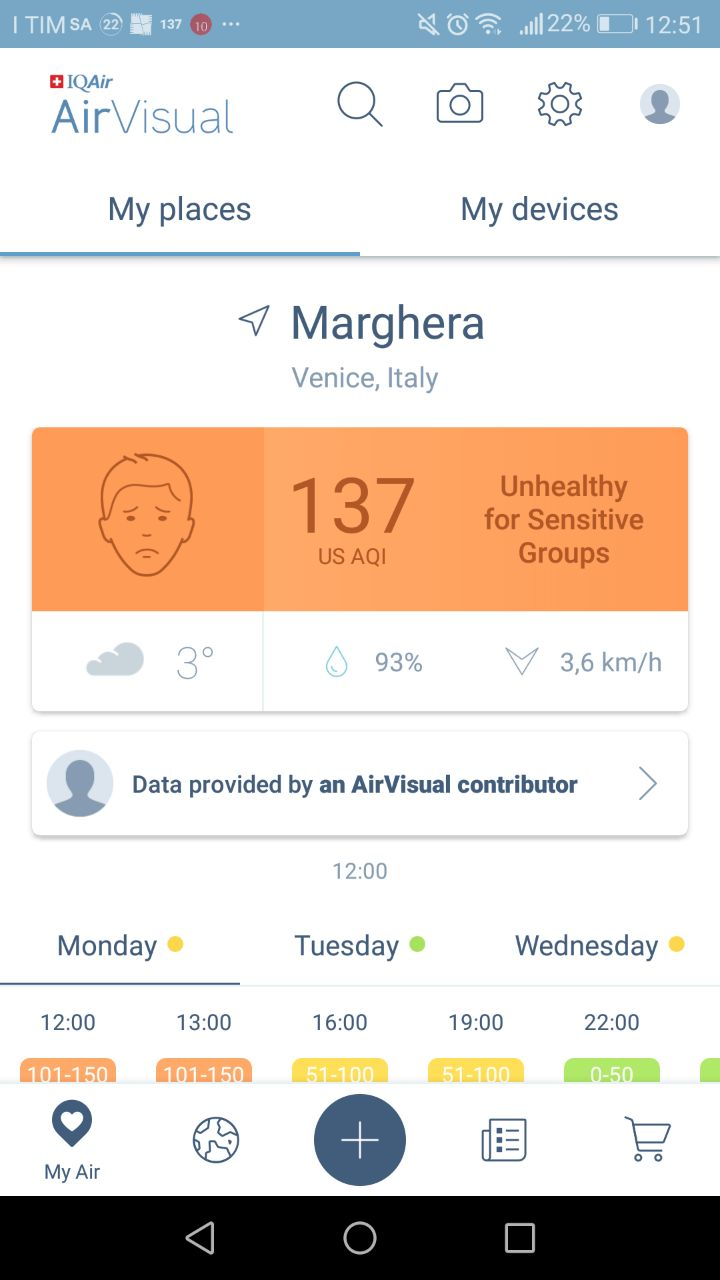
\includegraphics[width=4cm,height=10cm,keepaspectratio]{img/AirVisual1.jpeg}
  \hspace{0.1\textwidth}
  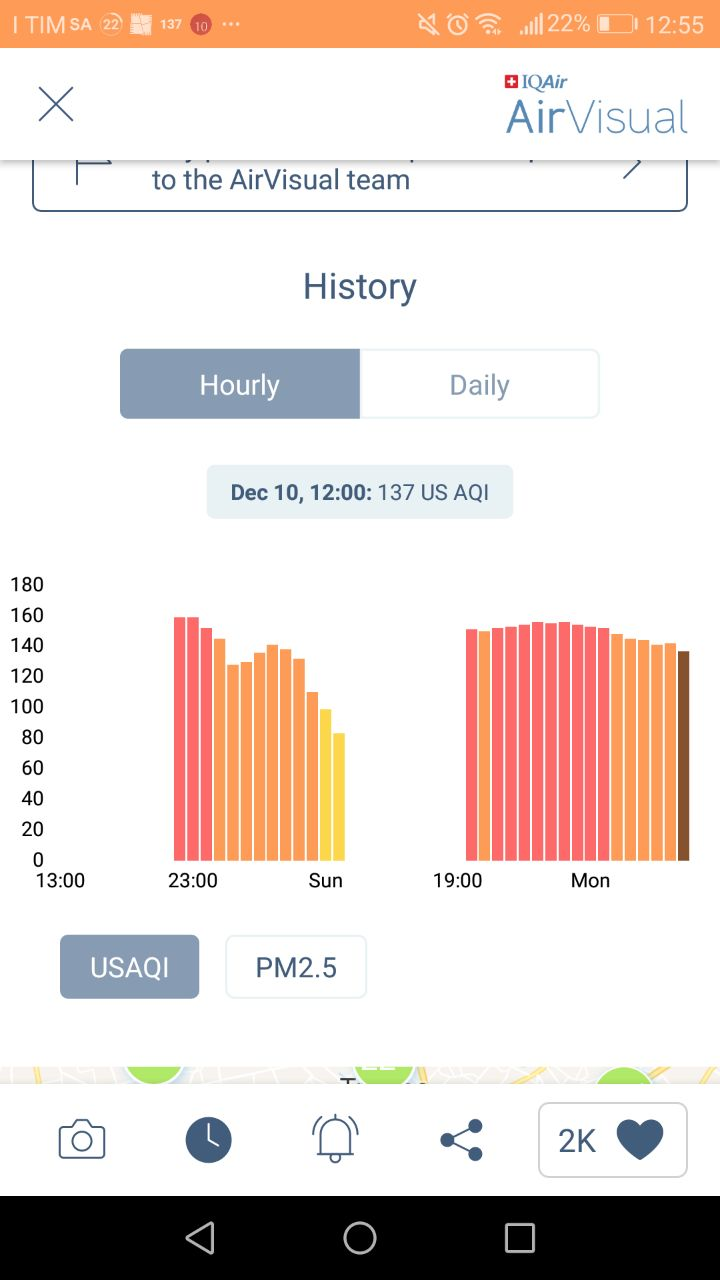
\includegraphics[width=4cm,height=10cm,keepaspectratio]{img/AirVisual2.jpeg}
  \hfill
  \caption{As we can see, the left most img has a 2-card design(My places/My devices), while the right most
  has a daily/hourly historic data.}
  \label{fig:boat4}
\end{figure}


\subsubsection{Air Quality:Real Time AQI}
From this app, we found really interesting the data visualization through histogram diagram and they visualize the data in a certain timespan.
\begin{figure}[H]
  \centering
  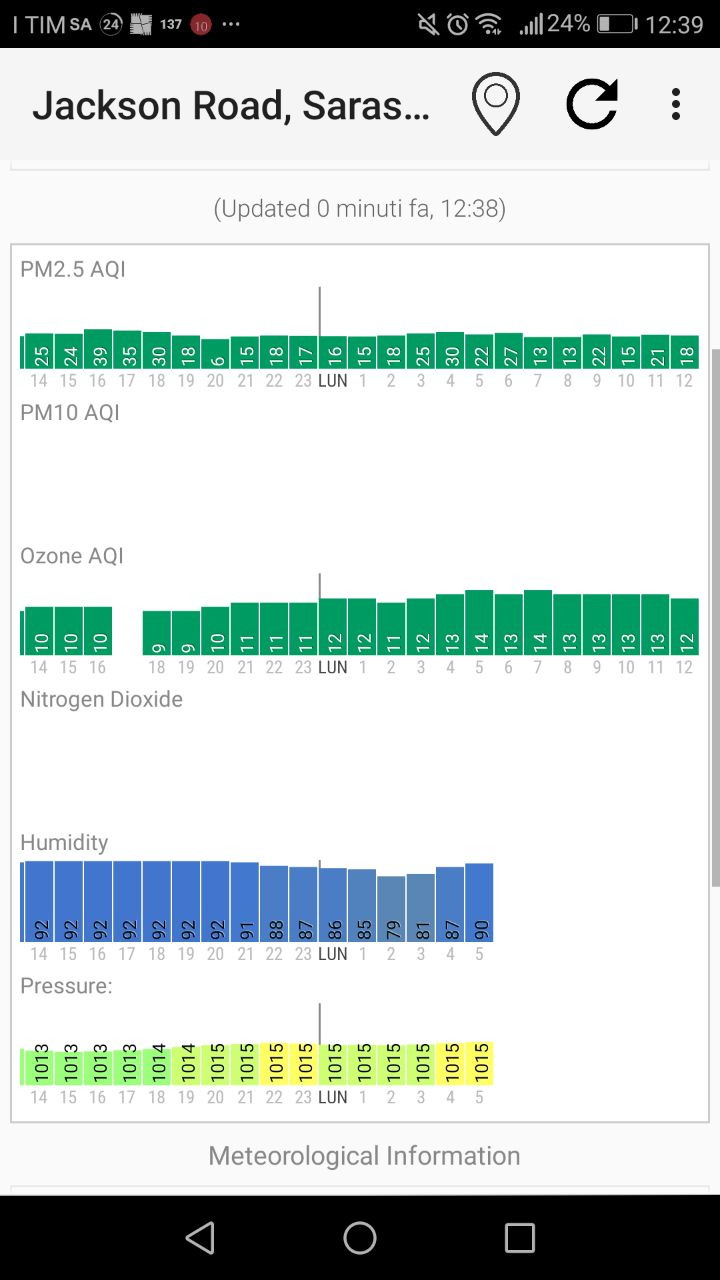
\includegraphics[width=4cm,height=10cm,keepaspectratio]{img/apphistogram.jpeg}
  \caption{Airquality histograms}
  \label{fig:boat3}
\end{figure}

\subsection{Technical Interface}
For the technical we searched for desktop online application and sites which treated the same kind of data(meteorologic, air pollution).

\subsubsection{acqin.org}
The site displays a large map with colored indicators that indicate the quality of the air in zone where the centers are placed. The use of colours permits a good comparison among the various centers.
\begin{figure}[H]
  \centering
  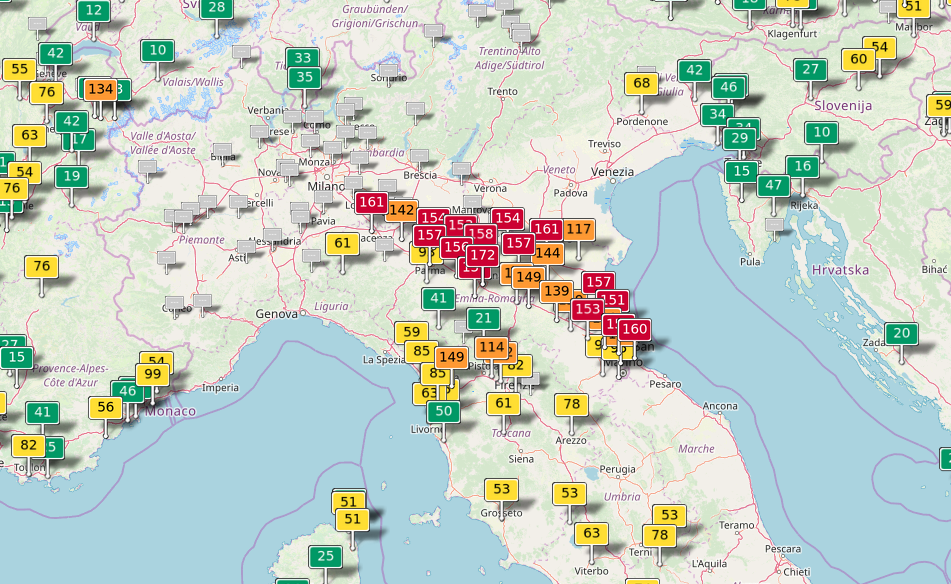
\includegraphics[width=25cm,height=10cm,keepaspectratio]{img/aqicn.png}
  \caption{acqin.org Labeled mapchart with the index of air pollution(the more polluted, the more the label is coloured red)}
  \label{fig:boat3}
\end{figure}
\subsubsection{waqi.org}
In this second app we have more types of data representation than before. We have a close-up on a specific location with the data relative to it represented in various formats!
\begin{figure}[H]
  \centering
  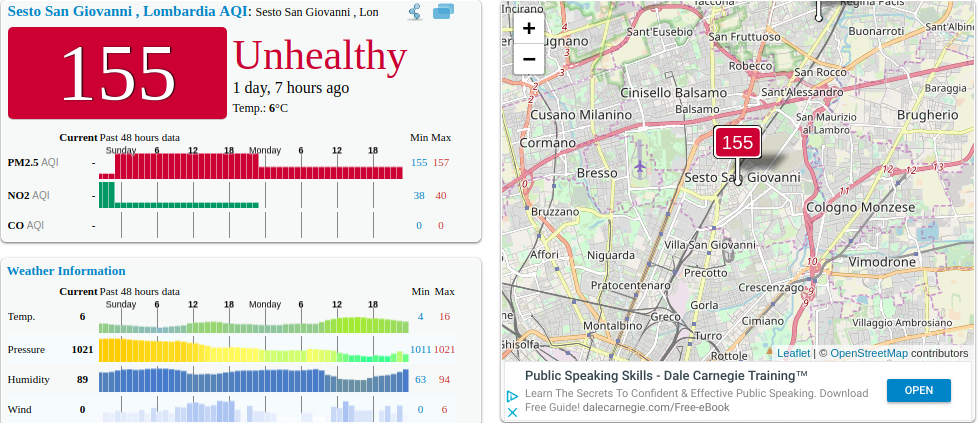
\includegraphics[width=15cm,height=10cm,keepaspectratio]{img/TechnicalExample.png}
  \caption{waqi.org in a example postion, which enhance the quality and quantity of data displayed}
  \label{fig:boat3}
\end{figure}

\end{itemize} 
\section{Proposal}
The solution provided will present the following representation. 
\subsection{Individual}
\subsubsection{Requirements}
We define here the requirements for the personal interfaces we decided to implement.
The smartphone app we were going to design must fulfill some requisites:
\begin{enumerate}
	\item Summarize all the information in an easy-to-use tool.
	\item Provide readable data about the behavior of a certain variable in time.
	\item Allow the most curios users to confront data between the/some stations.
\end{enumerate}
Build such a thing is not an easy task, given that the space is small and so you have to optimize it, to display in the best quality possible those data that the users
expect to see.
The smartwatch app cannot be as full of details as the smatphone's, given the more restricted space, it will only visualize the last measurements and a  daily history.
\subsubsection{Reasoning about the dataset}
Given the variables the station is measuring and what has to be shown through the interfaces, we have defined a simple hierarchy of the information.
We decided to divide them in two groups:
\begin{description}
\item Variables strongly dependent on location, and immutable/less important data
	\begin{itemize}	
	\item Weather(and Pressure)
	\item Hour, season
	\item Wind direction
	\item Location features
	\end{itemize}
\item Important variables, more likely to be studied and with some kind of behaviour
	\begin{itemize}
	\item CO2 ppm
	\item Wind speed
	\item Luminosity
	\item Temperature
	\item Umidity
	\item Rain
	\end{itemize}
\end{description}
We started building the interfaces based on this hierarchy, given more details for the most important variables.
\subsubsection{Smartphone Proposal}
The solution provided has to take into consideration that it has to give an easy representation of complex data. It is divided in two macroparts, a summary of the station first-group data and a view in detail of the most important variables.
The station is automatically selected if it's in the proximity of the device, otherwise it will be chosen by the user through a map.


\begin{figure}[H]
  \centering
  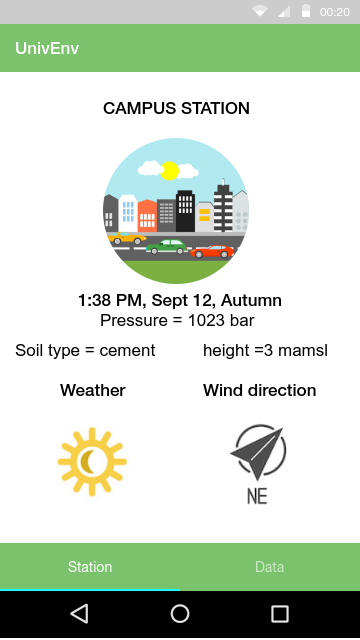
\includegraphics[width=4cm,height=10cm,keepaspectratio]{img/StationSummary.png}
  \hspace{0.1\textwidth}
  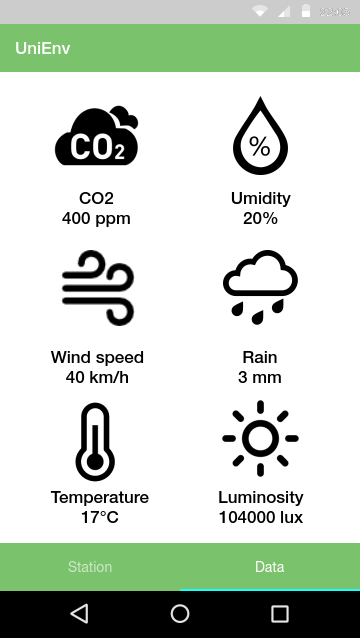
\includegraphics[width=4cm,height=10cm,keepaspectratio]{img/DataActivity.png}
  \hfill
  \caption{Smartphone activity}
  \label{fig:boat1}
\end{figure}

\subsubsection{User interaction}
INVISION LINK: https://invis.io/M5PI3T9Z3JX.

At the opening of the app, three things can happen
\begin{enumerate}
    \item The user is not in the proximity of a eco station, so a map will be visualized with the nearest ecostation(1-2 km range) and the user will choose what station visualize
    \item The user is near a station, presses the notification, the app will open up and the air condition activity of that particular  will open up
    \item The user is near a station, opens the app in the standard way and a popup will show up(You are near to "Vega ecostation", connect to it?).
\end{enumerate}


When a station is selected, the general display of that station will be visualized, that contains:
\begin{itemize}
\item Station name
\item Time and season
\item Weather around that particular station
\item Type of soil and enviroment
\item Height in maslm
\end{itemize}

If the user presses the data button, the icons of the most important variable will show up, with their current lecture already visible.

When an icon is pressed, the activity of that certain variable will popup up, in which the user can see how the last lecture approaches the annual max measure of that particular variable, as well as the behaviour of that variable in time(daily, monthly or annualy).

If the "Comparison" button is pressed, another activity will show up, which presents the comparison of actual lectures of the nearest stations and their behaviour in a week timespan.
The user can return to the menu with the left top screen error on the variable-related activity


\subsubsection{Graphs used}
\begin{itemize}
\item \textbf{Map Chart}

This will permit at a user which is not at beacon-range distance to a station to choose a station within a 2 km range max 

\item \textbf{Gauge chart}

It gives a representation to the max value registered in the season.

\item \textbf{Histogram chart}

We use this to show the history of a variable with different time ranges and an easy confrontation of last measure by different stations

\item \textbf{Line chart}

It confront the lectures of the different station within a week time span.
\end{itemize}



\subsubsection{Smartwatch}
\begin{figure}[H]
  \centering
  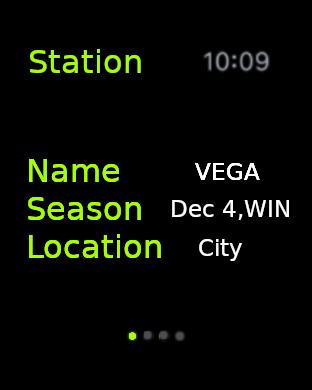
\includegraphics[width=4cm,height=10cm,keepaspectratio]{img/STATIONAW.png}
  \hspace{0.05\textwidth}
  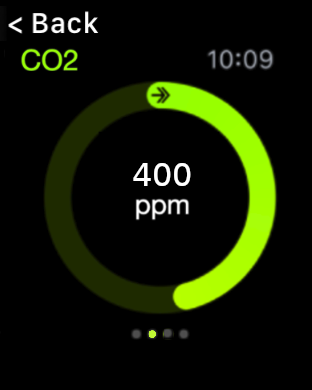
\includegraphics[width=4cm,height=10cm,keepaspectratio]{img/CO2AW.png}
  \hspace{0.05\textwidth}
  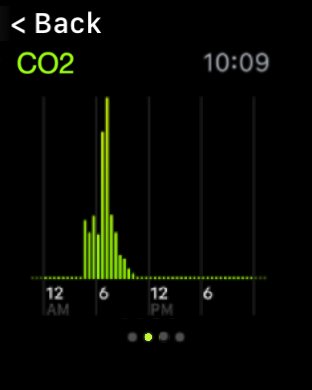
\includegraphics[width=4cm,height=10cm,keepaspectratio]{img/histoAW.png}
  \hfill
  \caption{Smartphone activity}
  \label{fig:boat1}
\end{figure}
INVISION link: https://invis.io/6HPIZVO7FNE.
For the smartwatch, which is a simple device, we decided not to provide lots of data or difficult plots that might result not clear to the user.
We represent only the most important variables, with a little overview of the location of the station, which is represented with a \textit{Modular Large Complication}.

The navigation of the app will be a \textit{page-based one}, with a total of 7 pages (one for each important variable plus 1 for station overview).
The user can swipe through the pages, and in a page representing a variable, a double tap on the radar chart can change the type of data representation the page will visualize.

\subsubsection{Graphs used}
\begin{itemize}
\item \textbf{Radial bar chart}

We use it to visualize the current variable measurement with respect to a daily/montly/annual max value
\item \textbf{Histogram chart}

Is a simple plot that can give a quick view to a short history of the variables, in order to extract possible behaviors of a certain variable.
\end{itemize}
\subsection{Public}
The public interface has been structured in two parts. 
\begin{itemize}
\item The first screen (Figure 2), is an image that represent the current state of our  environment depending on the variables defined before. If, for example, the level of CO2 is over the average level, we'll add some smog clouds in our representation. Now we define, for each variable, what we are going to add if the level is over the normal level. The temperature is given by a string in the upper-right part.
\begin{itemize}
\item CO2: smog clouds.
\item Air Humidity: fog.
\item Luminosity: bigger sun.
\item Wind speed and direction: wind icon and clouds.
\item Location (also height, type of soil, type of surrounding environment): is described by the image.
\item Time (hour/season): there is a string indicating what time is it. For the season, it's described by the image.
\item Pressure: arrows going down
\item Rain: clouds with rain
\end{itemize} 

This representation is thought to be as abstract as possible, in order to be accessible to all people (e.i. kids, adults, etc).
There'll be a sound output that will tell you what you are clicking, for helping blind people.

\begin{figure}[H]
  \centering
  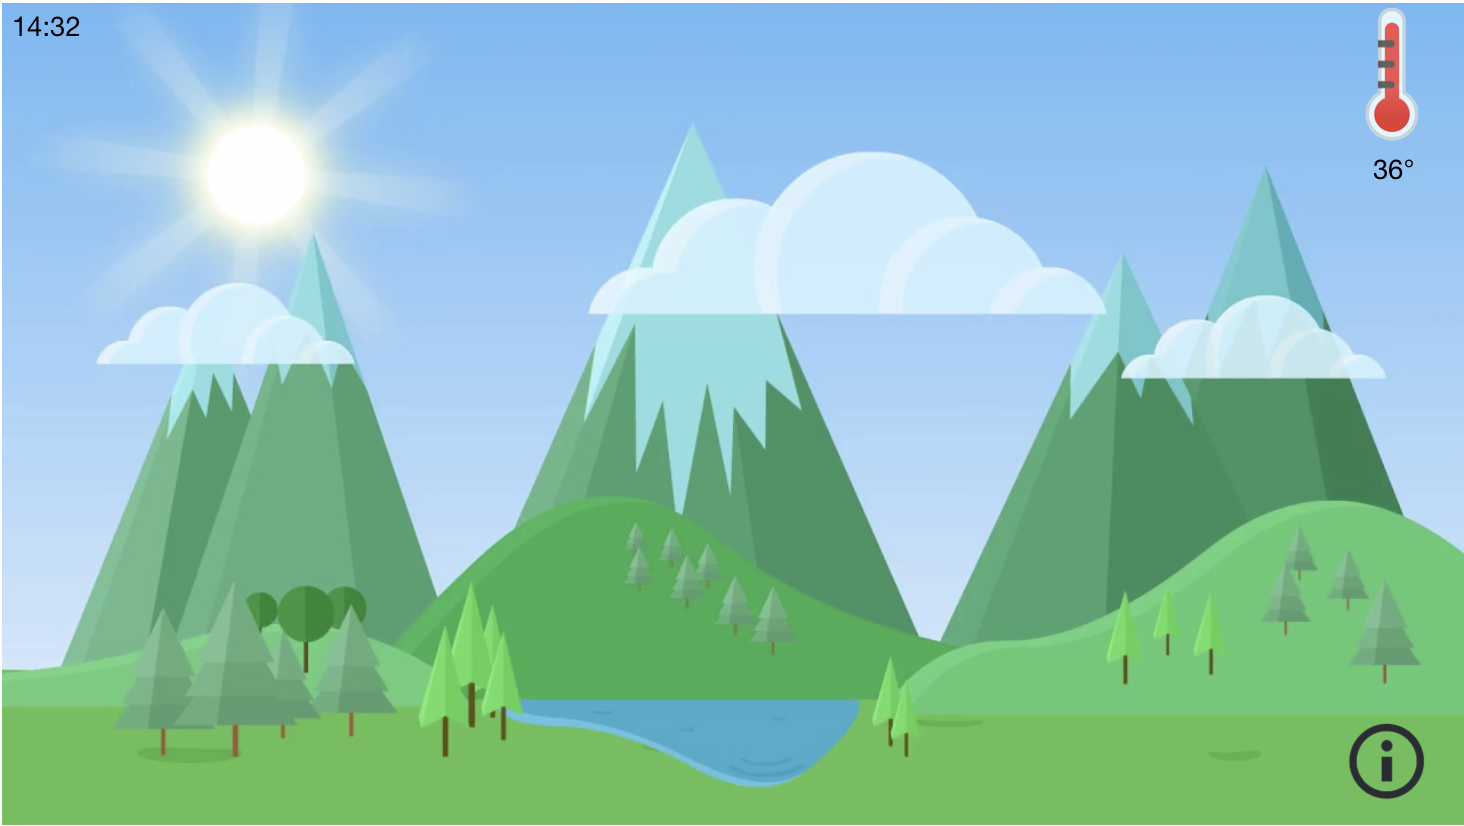
\includegraphics[width=4cm,height=10cm,keepaspectratio]{img/p1.png}
  \caption{Public interface}
  \label{fig:boat1}
\end{figure}
\begin{figure}[H]
  \centering
  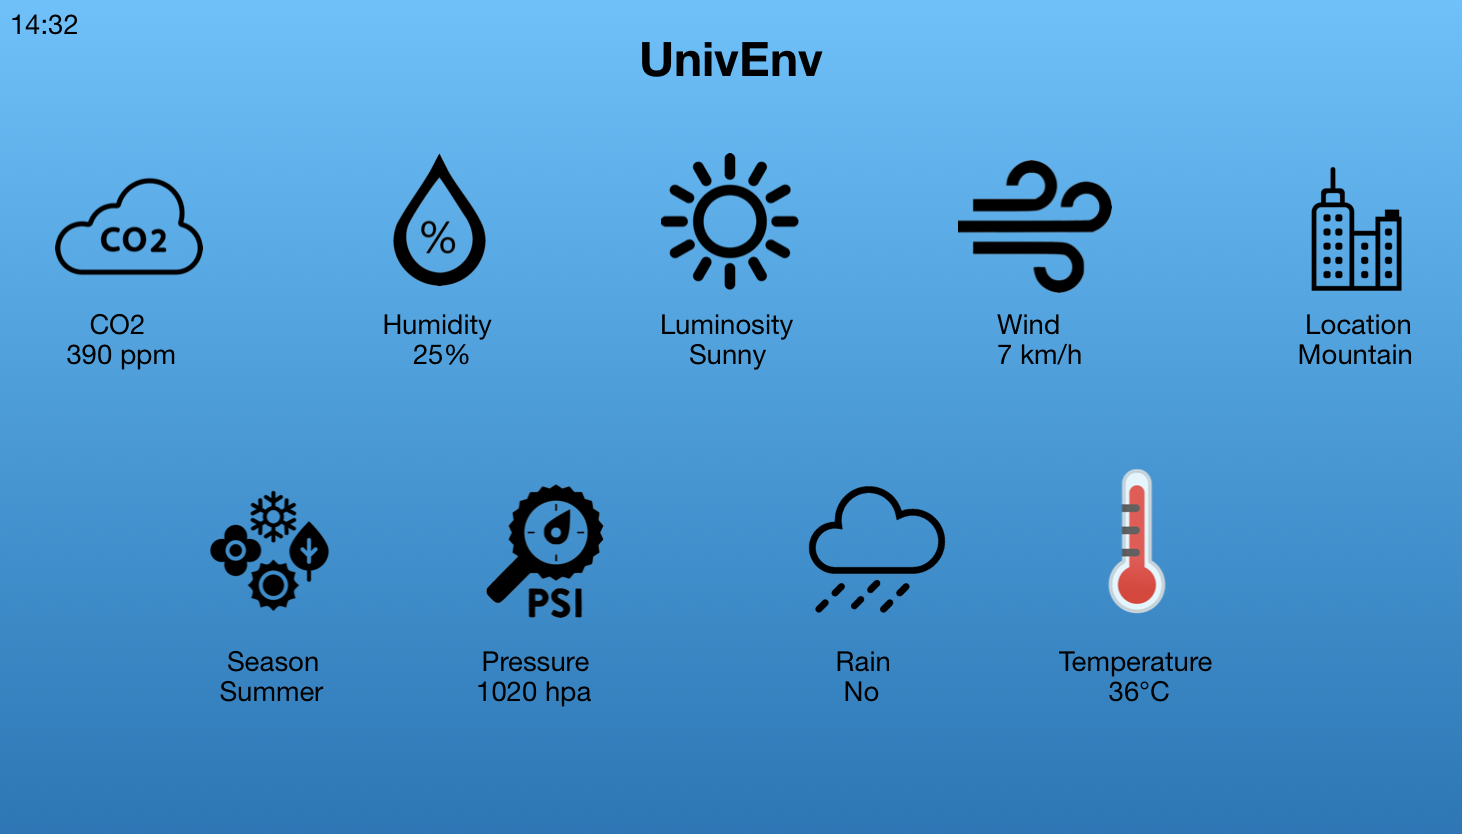
\includegraphics[width=0.4\textwidth]{img/p2.png}
  \caption{Info of public interface}
  \label{fig:boat2}
\end{figure}
\end{itemize}
\newpage
\subsection{Technical}
INVISION link: https://invis.io/3WPJB0OEYAP.
This type of representation is for people that analyze the row data, so it has been chosen to use representations that maybe are less intuitive to understand but are more accurate. \\ It has also been introduced the comparison, which allows to select the type of data to compare, and compare it.
The system is divided in the following parts: 
\begin{itemize}
\item Login
\item Representation
\item Choice of what compare  
\item Comparison
\end{itemize}
It has been chosen the following type of representation: 
\begin{itemize}
\item Scatter chart
\item Colored intensity map
\item Trend line
\item Point representation with mean
\item Radar chart
\end{itemize}
The following mockup represent the system that will be used by technicians.\\
\begin{figure}[H]
  \centering
  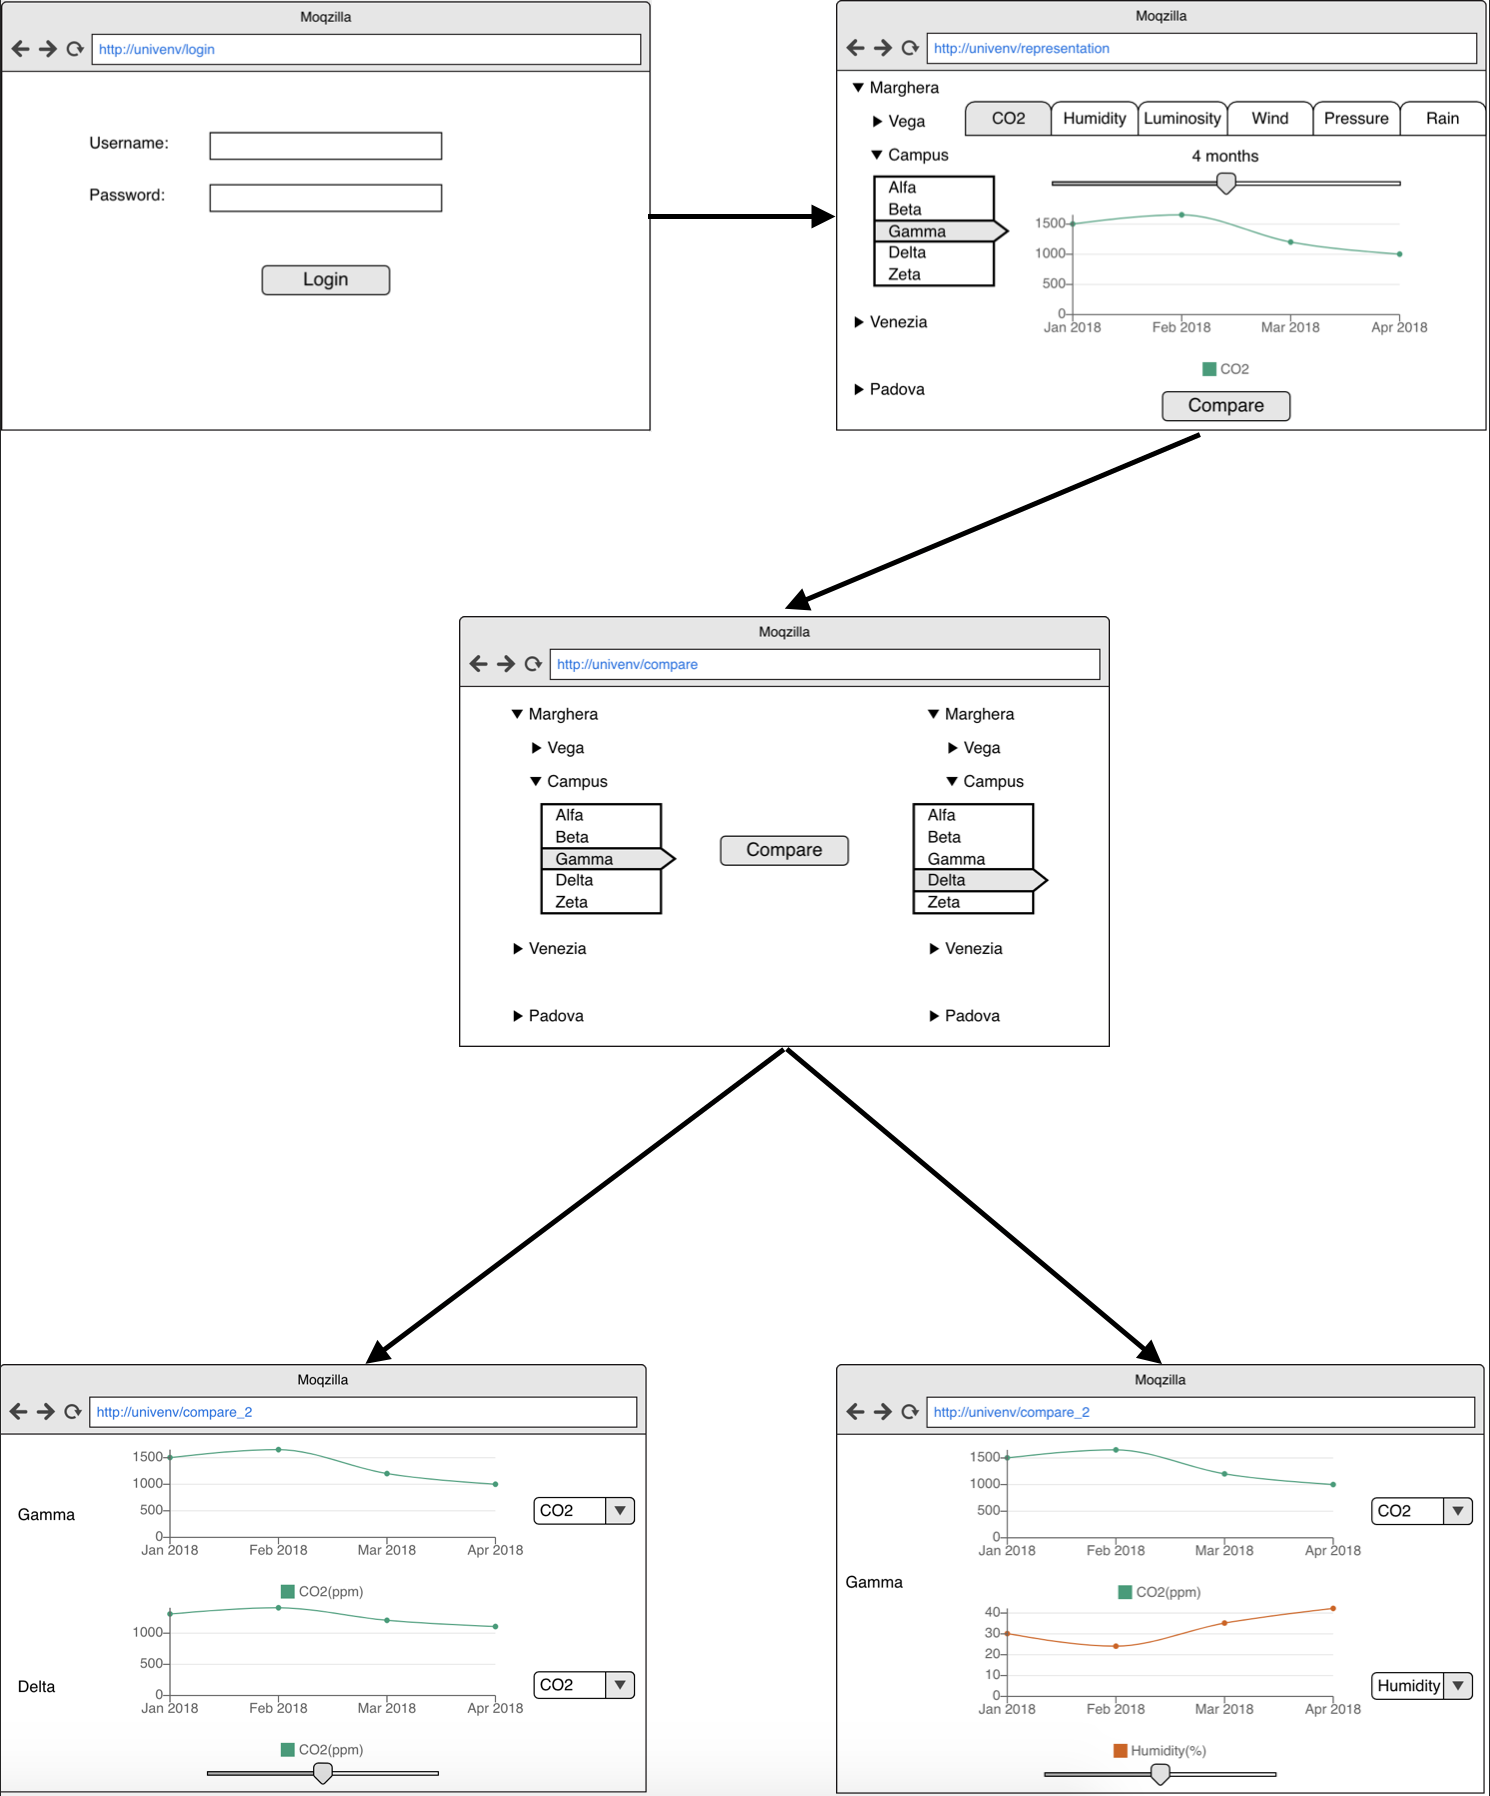
\includegraphics[width=1\textwidth]{img/tot.png}
  \caption{Technical interface}
  \label{fig:boat1}
\end{figure}
\subsection{Type of graphs}
It has been chosen those type of representation because they represent accurately the raw data. The exceptions are the radar chart, it has been chosen because it sum up all the variables(the values goes from 0 to 10, which represent the quality of that variable); and the colored intensity map which represent the situation in that moment on the map. 
\begin{figure}[H]
  \centering
  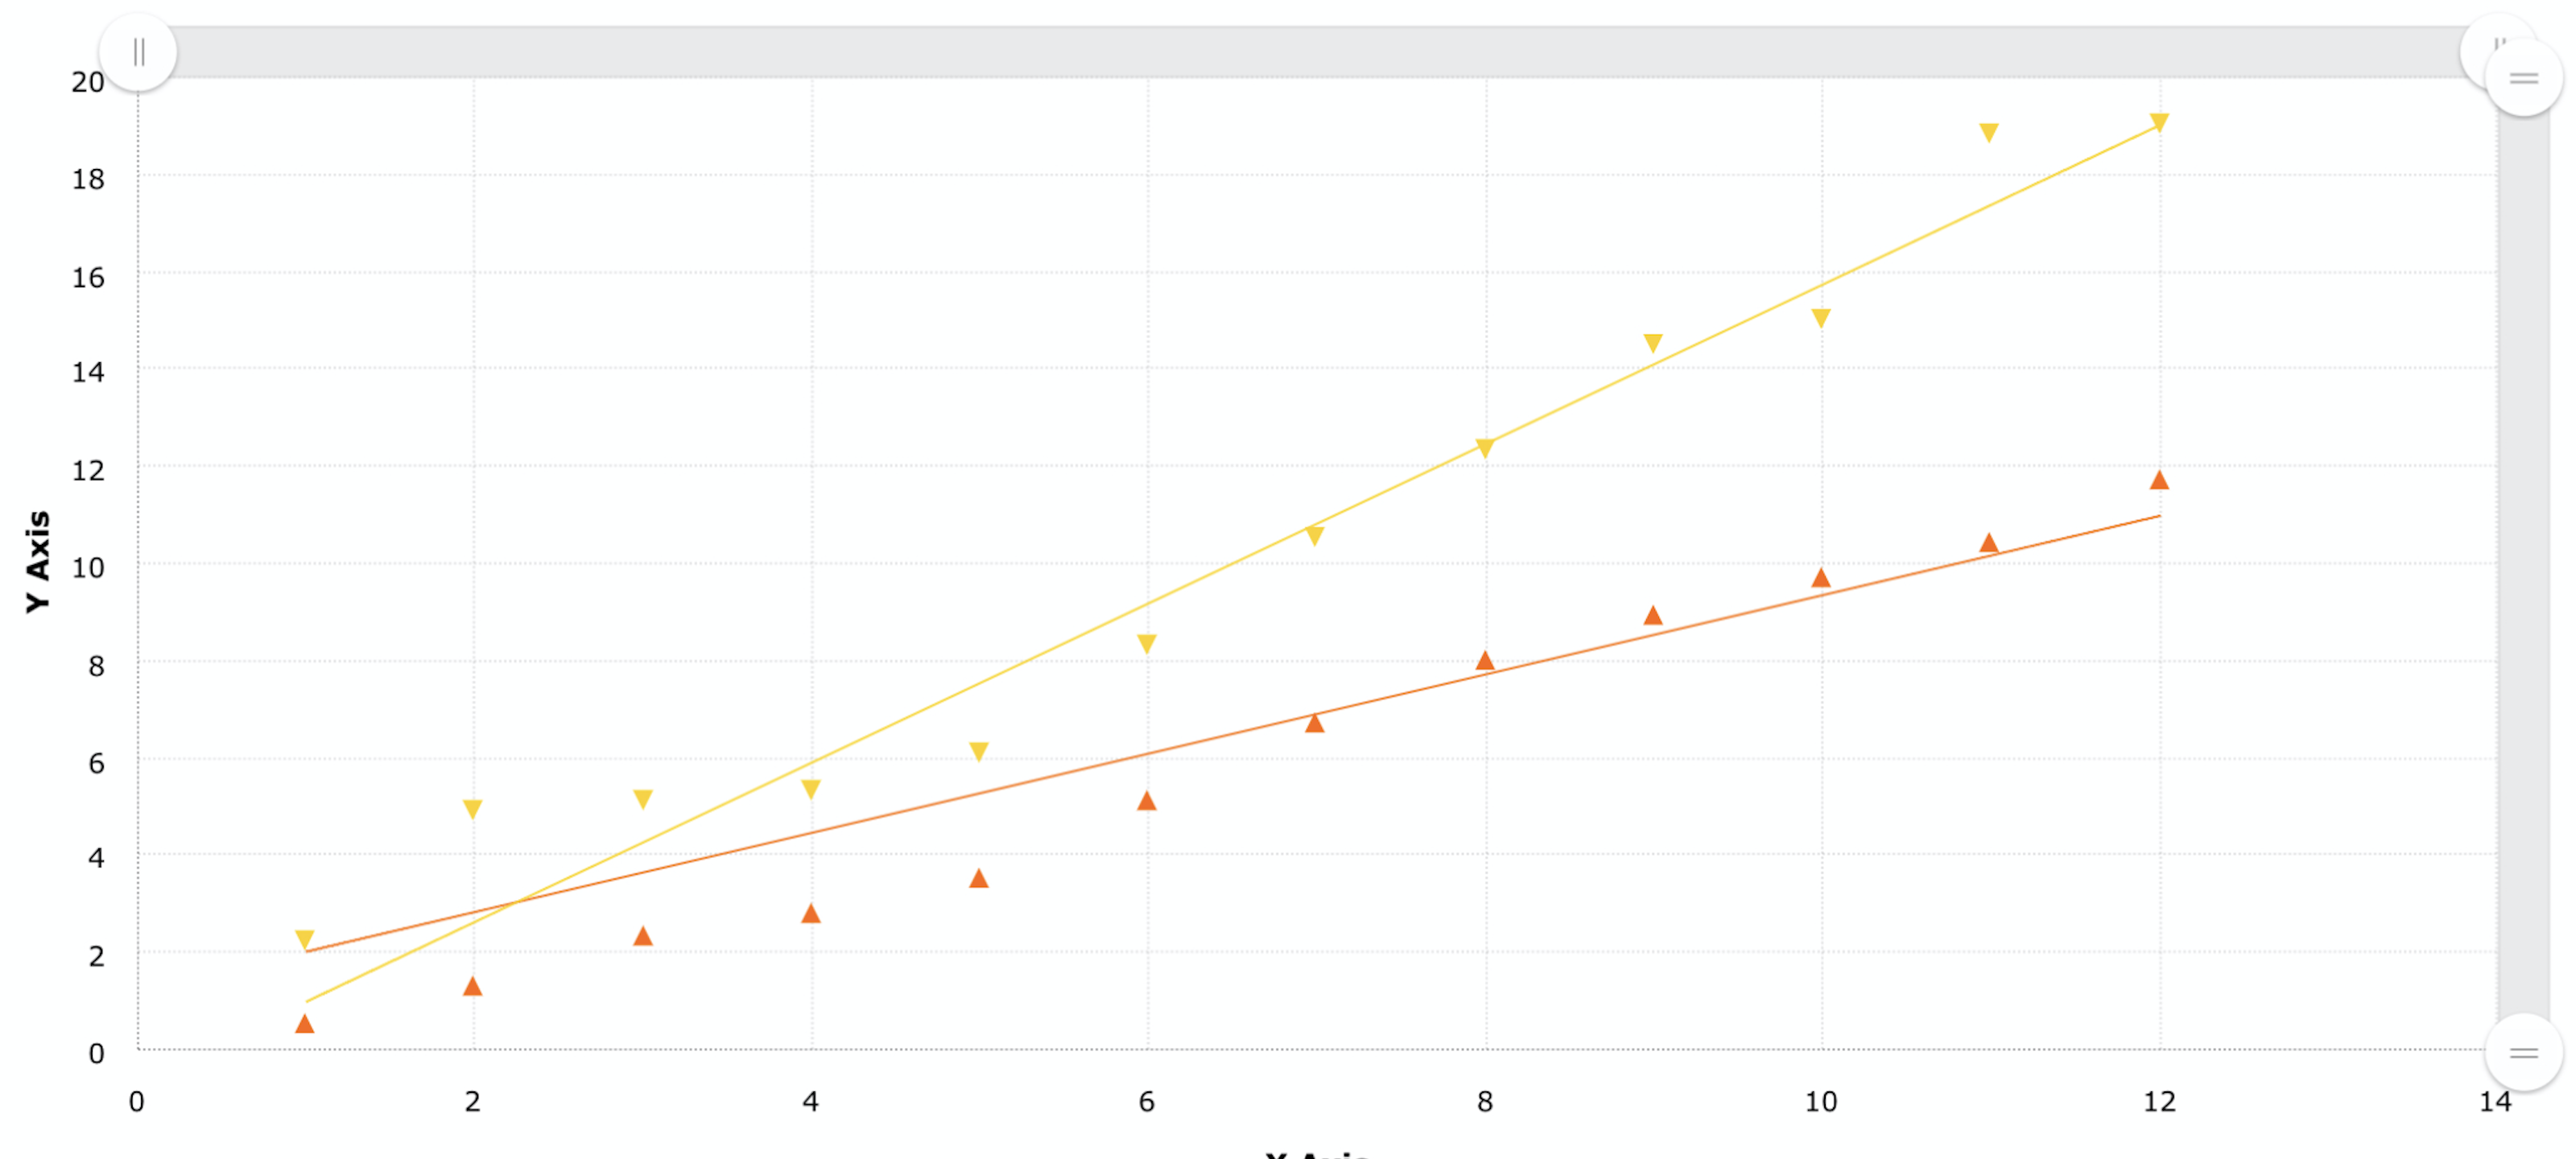
\includegraphics[width=0.7\textwidth]{img/scatter_chart.png}
  \caption{Scatter chart}
  \label{fig:boat1}
\end{figure}
\begin{figure}[H]
  \centering
  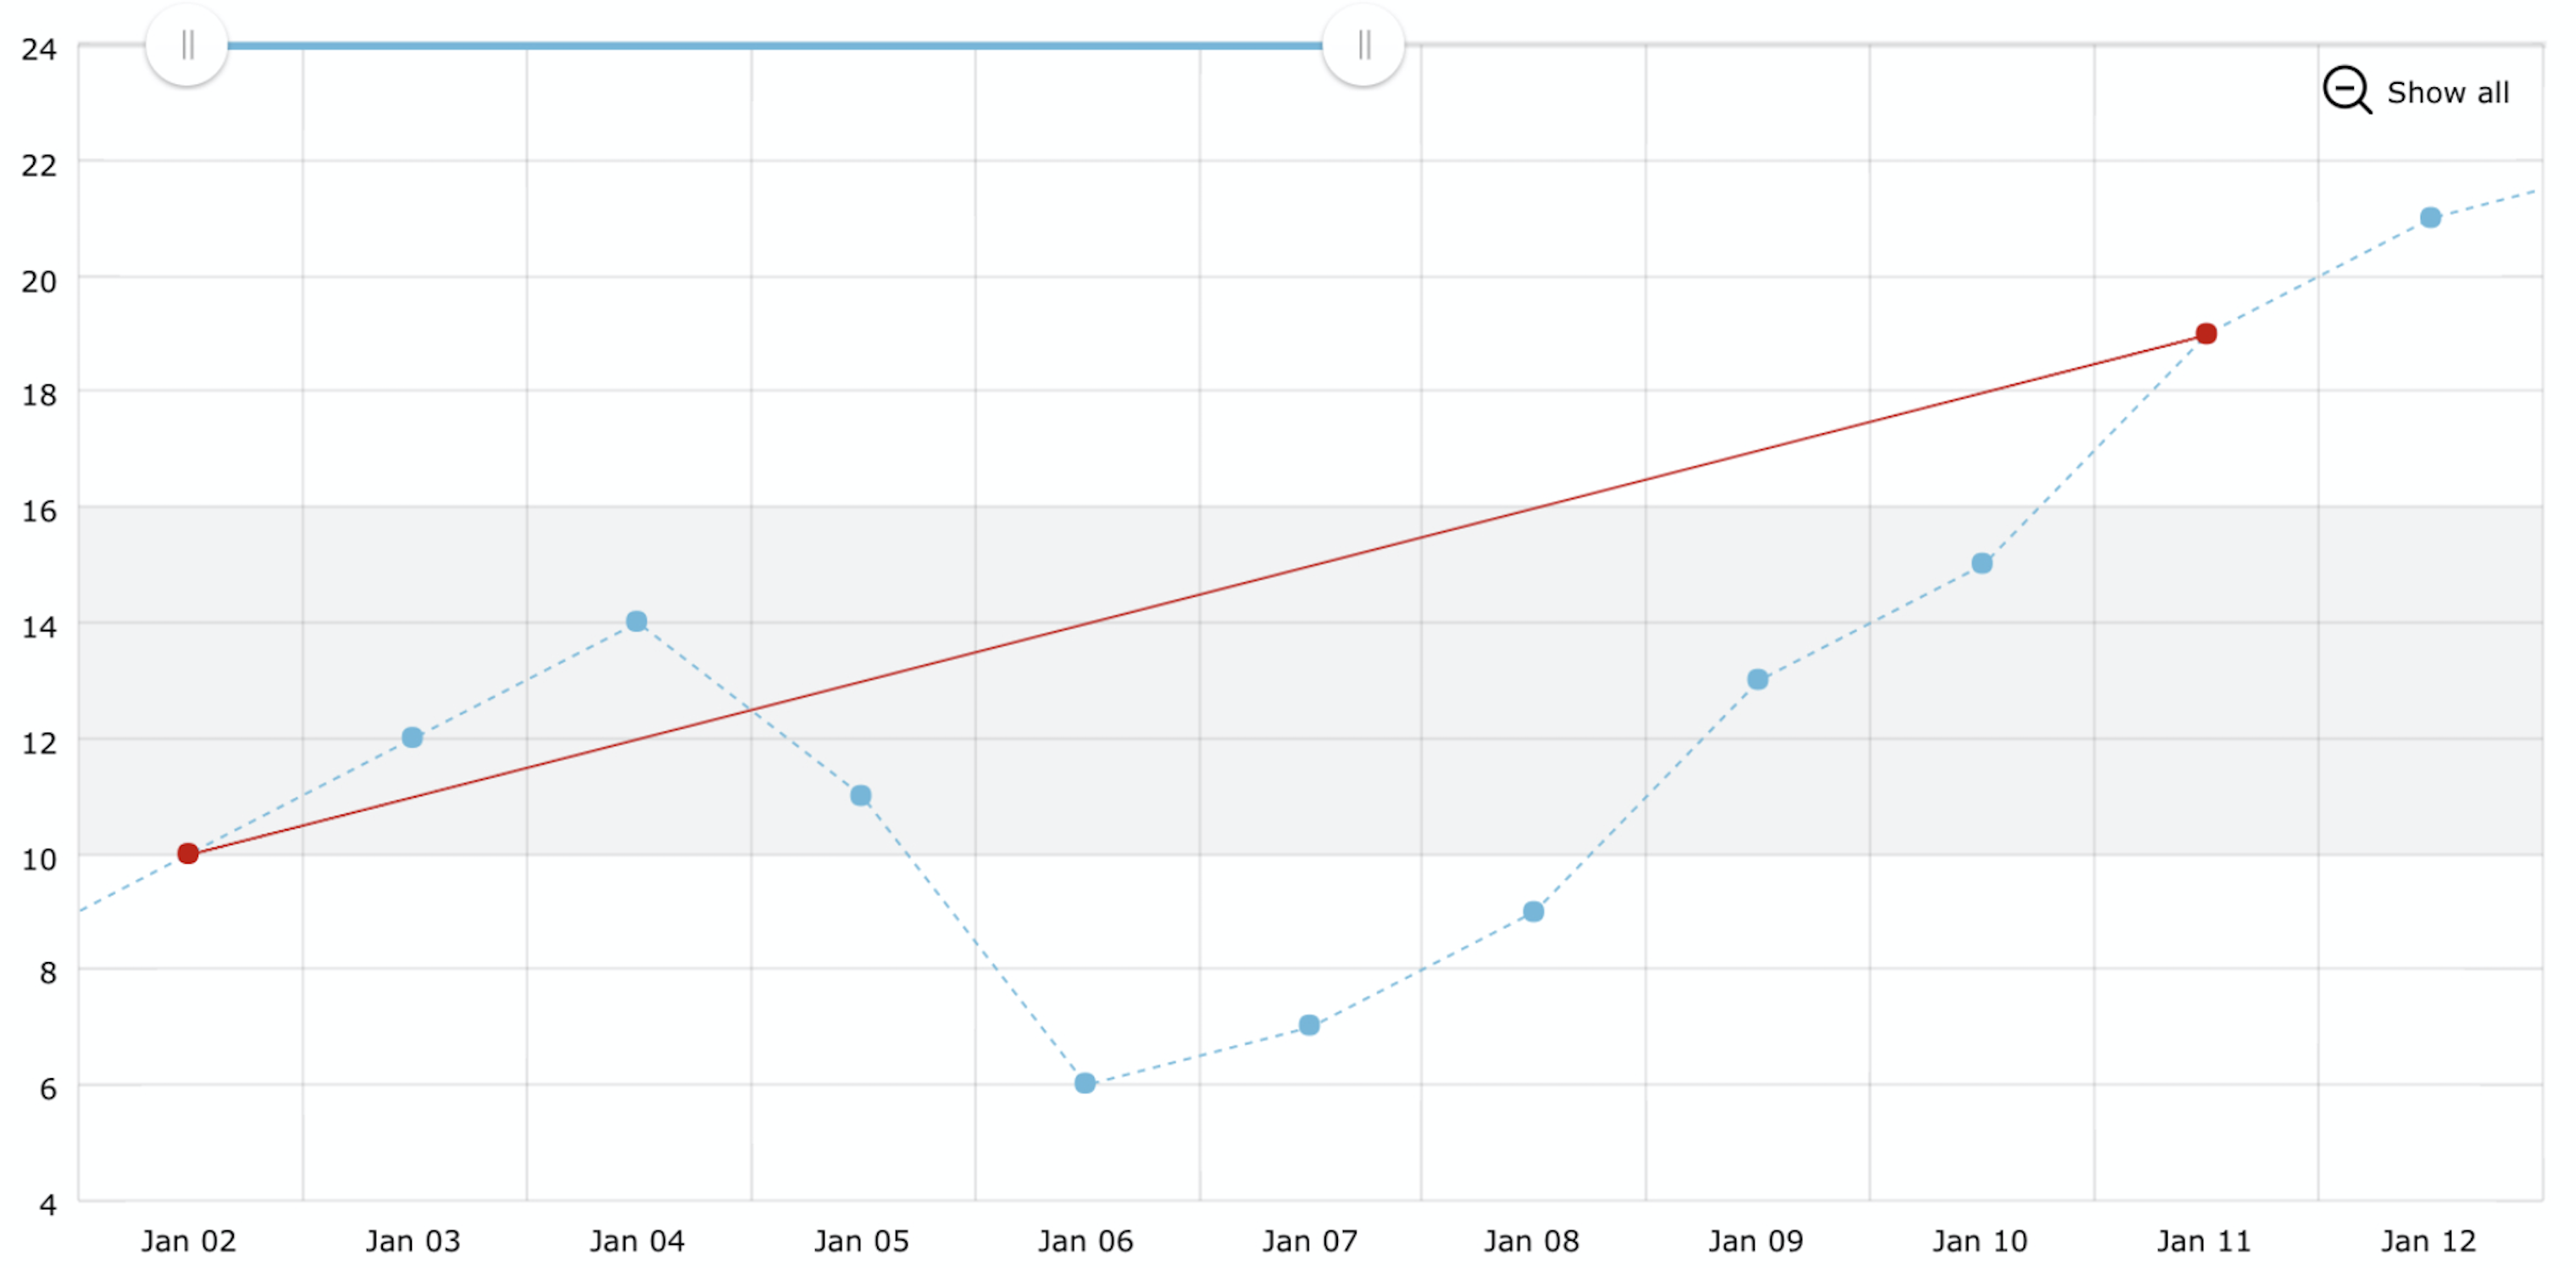
\includegraphics[width=0.7\textwidth]{img/trend_line.png}
  \caption{Trend line}
  \label{fig:boat1}
\end{figure}
\begin{figure}[H]
  \centering
  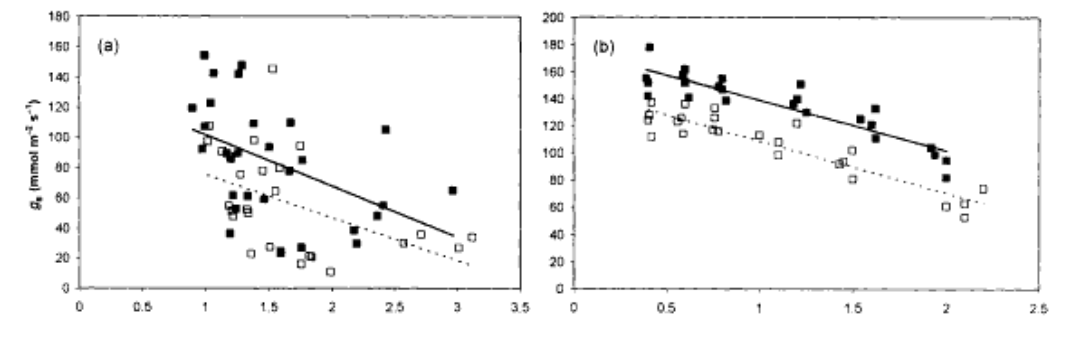
\includegraphics[width=0.6\textwidth]{img/point.png}
  \caption{Scatter Point representation with mean line}
  \label{fig:boat1}
\end{figure}
\begin{figure}[H]
  \centering
  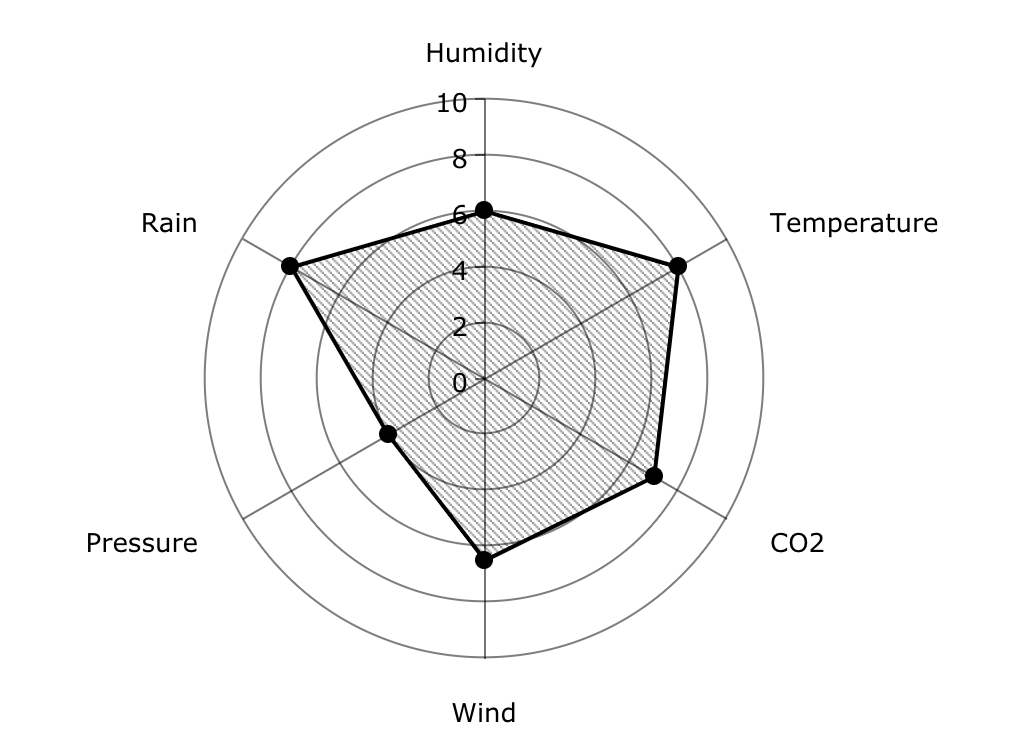
\includegraphics[width=0.6\textwidth]{img/dont_know.png}
  \caption{Radar graph}
  \label{fig:boat1}
\end{figure}
\begin{figure}[H]
  \centering
  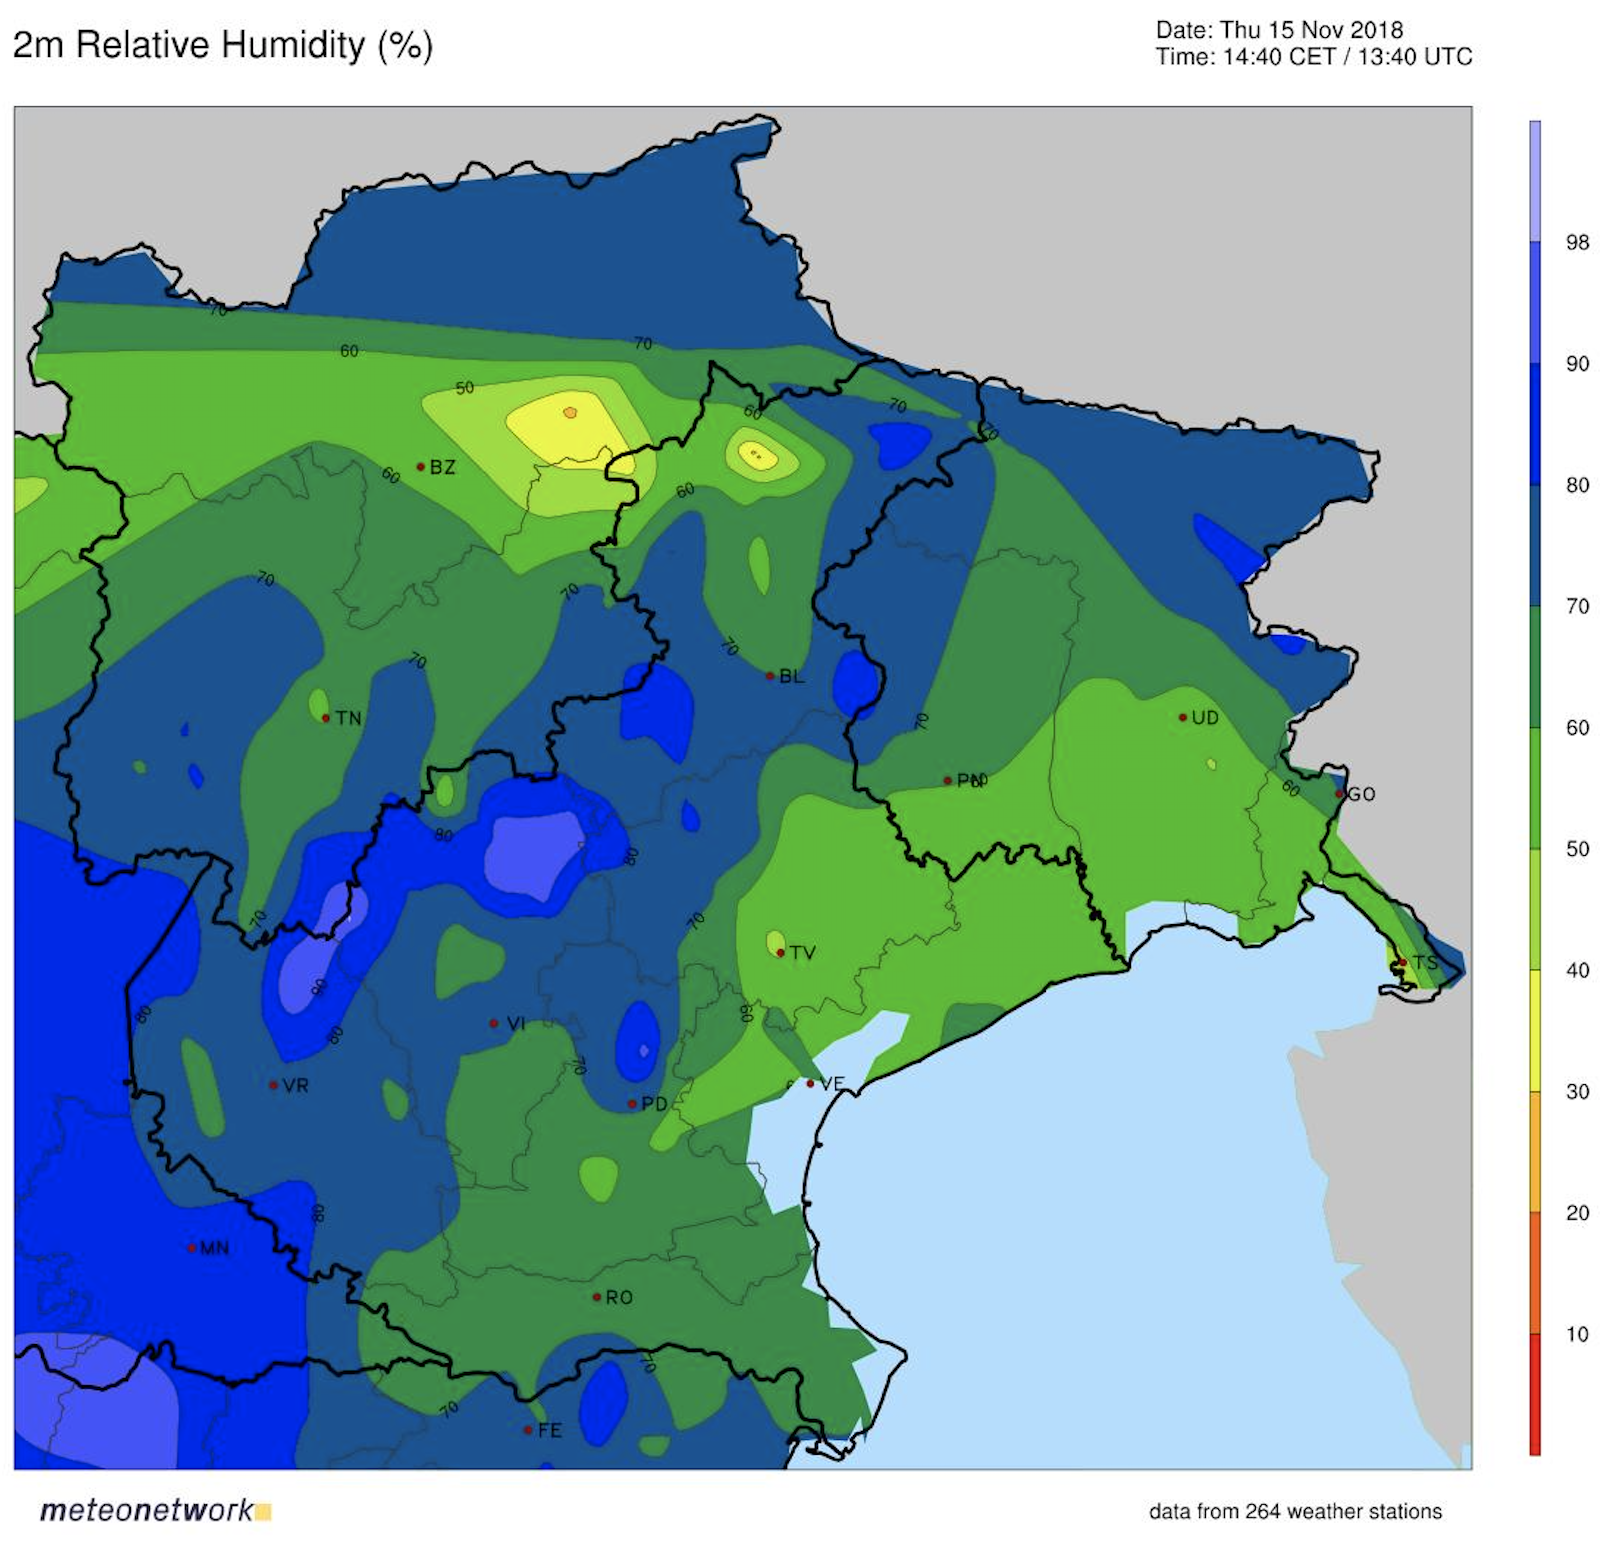
\includegraphics[width=0.4\textwidth]{img/lol.png}
  \caption{Colored intensity map}
  \label{fig:boat1}
\end{figure}

\newpage
%----------------------------------------------------------------------------------------
%	BIBLIOGRAPHY
%----------------------------------------------------------------------------------------
\section{Bibliography}
\begin{thebibliography}{99} % Bibliography - this is intentionally simple in this template

\bibitem B. E. Medlyn, C. V. M. Barton, M. S. J. Broadmeadow, R. Ceulemans{art}
Stomatal Conductance of Forest Species after Long-Term Exposure to Elevated CO2 Concentration: A Synthesis;
\newblock {The New Phytologist, vol. 149, n. 2, Feb. 2001.},  pp. 247-264.

\bibitem {}
Apple,\\ Human Interface Guidelines, Gestures; \\
\newblock {https://developer.apple.com/design/human-interface-guidelines/watchos/user-interaction/gestures/}

 
\end{thebibliography}

%----------------------------------------------------------------------------------------

\end{document}